\documentclass[a4paper]{article}
\usepackage[warn]{mathtext}
\usepackage[utf8]{inputenc}
\usepackage[T2A]{fontenc}

\usepackage[english,russian]{babel}
\usepackage{multicol}
\usepackage{fancyhdr}
\usepackage{graphicx}
\usepackage{microtype}
\usepackage{wrapfig}
\usepackage{amsmath}
\usepackage{floatflt}
\usepackage{geometry} \geometry{verbose,a4paper,tmargin=2cm,bmargin=2cm,lmargin=1.5cm,rmargin=1.5cm}
\usepackage{float}
\usepackage{amssymb}
\usepackage{caption}
\usepackage{epsfig}
\usepackage{newunicodechar}


\usepackage{listings}
\usepackage{color}

\definecolor{dkgreen}{rgb}{0,0.6,0}
\definecolor{gray}{rgb}{0.5,0.5,0.5}
\definecolor{mauve}{rgb}{0.58,0,0.82}

\lstset{
  language=Java,
  aboveskip=3mm,
  belowskip=3mm,
  showstringspaces=false,
  columns=flexible,
  basicstyle={\small\ttfamily},
  numbers=none,
  numberstyle=\tiny\color{gray},
  keywordstyle=\color{blue},
  commentstyle=\color{dkgreen},
  stringstyle=\color{mauve},
  breaklines=false,
  breakatwhitespace=true,
  tabsize=3
}

\begin{document}

\graphicspath{ {pictures/} }

\begin{titlepage}
	\centering
	\vspace{5cm}
    {\scshape\LARGE NetCracker Learning center\par}
	\vspace{5cm}
	{\scshape\Large  Учебное практическое задание № 1 \par}
	\vspace{1cm}
    {\huge\bfseries  Задание 1. Объектно-ориентированно епрограммиорвание в Java \par}
	\vspace{1cm}
	\vfill
    \begin{flushright}
        {\large выполнил студент}\par
        \vspace{0.3cm}
        {\LARGE Яромир Водзяновский}
    \end{flushright}
	\vfill
Долгопрудный, 2021
% Bottom of the page
\end{titlepage}

\pagestyle{fancy} 
\fancyhead[L]{Java   $\sim  \hat(\, ^{\circ}  \omega  ^{\circ} \, \hat) \sim$}
\fancyhead[R]{NetCracker}
\fancyfoot[C]{ \noindent\rule{\textwidth}{0.4pt} \thepage }



\newpage


Код лежит на GitHub: 
\section{Задача 1}

\textbf{Цель:} Разработайте класс для решения квадратных уравнений. Вычисление дискриминанта должен осуществлять вложенный класс. После компиляции объясните структуру class файлов. Проанализируйте использование вложенного класса. \par


\begin{lstlisting}
    import java.util.Scanner;

    public class Solver {
    
        class Discr {
    
            public double discr_calc(int a, int b, int c) {
                double discr = b*b - 4*a*c;
                return discr;
            }
        }
    
        public static double[] answer(int a, int b, double discr) {
            double[] res = new double[2];
            for (int i=0; i<2; i++) {
                res[i] = (-b + Math.pow(-1, i) * Math.sqrt(discr)) / (2 * a);
            }
            return res;
        }
    
        public static void main(String[] args) {
    
            int[] coeffs;
            double[] answer = new double[2];
    
            Scanner in = new Scanner(System.in);
    
            coeffs = new int [3];
            for (int i=0; i<3; i++) {
                System.out.print("Enter coeff " + i + " : ");
                coeffs[i] = in.nextInt();
            }
            in.close();
    
            int a = coeffs[0];
            int b = coeffs[1];
            int c = coeffs[2];
    
            Solver solver = new Solver();
            Discr discr = solver.new Discr();
    
            double discriminante = discr.discr_calc(a, b, c);
    
            if (a == 0 && b == 0 && c == 0) {
            System.out.println("The Answer: Infinity amount of solutions!");
    
            } else {
                if (discriminante < 0) {
                    System.out.println("The Answer: No solution in Real numbers!");
                } else {
                    if (a == 0) {
                        double answer_linear = -c / b;
                        System.out.println("The Answer: " + answer_linear);
        
                    } if (a == 0 && b == 0 && c != 0) {
                        System.out.println("The Answer: No solution");
        
                    } if (a != 0) {
                    answer = answer(a, b, discriminante);
                    System.out.println("The Answer: " + answer[0] + " and " + answer[1]);
                    }
                }
            } 
        }
    }    
\end{lstlisting}

\begin{figure}[H]
    \begin{center}
        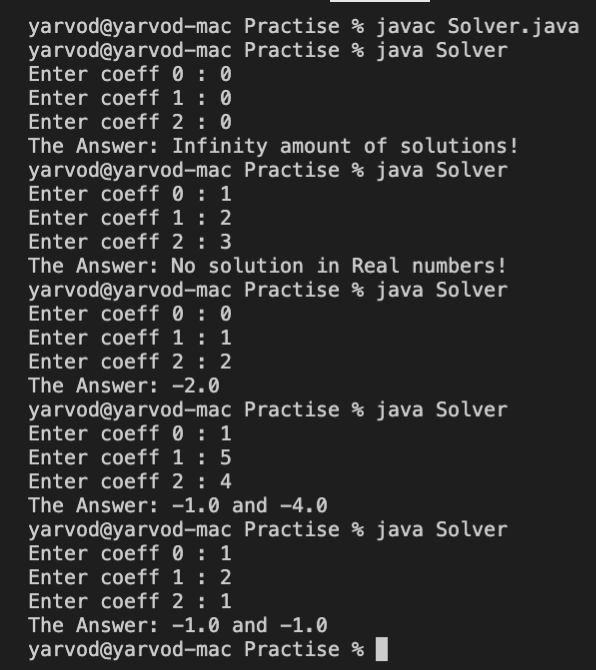
\includegraphics[scale = 0.5]{solution_1.png}
        \caption{Решение задачи 1}
        \label{sol_1}
    \end{center}
\end{figure}


\end{document}